\PassOptionsToPackage{unicode=true}{hyperref} % options for packages loaded elsewhere
\PassOptionsToPackage{hyphens}{url}
%
\documentclass[]{book}
\usepackage{lmodern}
\usepackage{amssymb,amsmath}
\usepackage{ifxetex,ifluatex}
\usepackage{fixltx2e} % provides \textsubscript
\ifnum 0\ifxetex 1\fi\ifluatex 1\fi=0 % if pdftex
  \usepackage[T1]{fontenc}
  \usepackage[utf8]{inputenc}
  \usepackage{textcomp} % provides euro and other symbols
\else % if luatex or xelatex
  \usepackage{unicode-math}
  \defaultfontfeatures{Ligatures=TeX,Scale=MatchLowercase}
\fi
% use upquote if available, for straight quotes in verbatim environments
\IfFileExists{upquote.sty}{\usepackage{upquote}}{}
% use microtype if available
\IfFileExists{microtype.sty}{%
\usepackage[]{microtype}
\UseMicrotypeSet[protrusion]{basicmath} % disable protrusion for tt fonts
}{}
\IfFileExists{parskip.sty}{%
\usepackage{parskip}
}{% else
\setlength{\parindent}{0pt}
\setlength{\parskip}{6pt plus 2pt minus 1pt}
}
\usepackage{hyperref}
\hypersetup{
            pdftitle={I am Bilingual - Python and R},
            pdfauthor={Priyanga Dilini Talagala   Thiyanga S. Talagala},
            pdfborder={0 0 0},
            breaklinks=true}
\urlstyle{same}  % don't use monospace font for urls
\usepackage{longtable,booktabs}
% Fix footnotes in tables (requires footnote package)
\IfFileExists{footnote.sty}{\usepackage{footnote}\makesavenoteenv{longtable}}{}
\usepackage{graphicx,grffile}
\makeatletter
\def\maxwidth{\ifdim\Gin@nat@width>\linewidth\linewidth\else\Gin@nat@width\fi}
\def\maxheight{\ifdim\Gin@nat@height>\textheight\textheight\else\Gin@nat@height\fi}
\makeatother
% Scale images if necessary, so that they will not overflow the page
% margins by default, and it is still possible to overwrite the defaults
% using explicit options in \includegraphics[width, height, ...]{}
\setkeys{Gin}{width=\maxwidth,height=\maxheight,keepaspectratio}
\setlength{\emergencystretch}{3em}  % prevent overfull lines
\providecommand{\tightlist}{%
  \setlength{\itemsep}{0pt}\setlength{\parskip}{0pt}}
\setcounter{secnumdepth}{5}
% Redefines (sub)paragraphs to behave more like sections
\ifx\paragraph\undefined\else
\let\oldparagraph\paragraph
\renewcommand{\paragraph}[1]{\oldparagraph{#1}\mbox{}}
\fi
\ifx\subparagraph\undefined\else
\let\oldsubparagraph\subparagraph
\renewcommand{\subparagraph}[1]{\oldsubparagraph{#1}\mbox{}}
\fi

% set default figure placement to htbp
\makeatletter
\def\fps@figure{htbp}
\makeatother

\usepackage{booktabs}
\usepackage{amsthm}
\makeatletter
\def\thm@space@setup{%
  \thm@preskip=8pt plus 2pt minus 4pt
  \thm@postskip=\thm@preskip
}
\makeatother
\usepackage[]{natbib}
\bibliographystyle{apalike}

\title{I am Bilingual - Python and R}
\author{Priyanga Dilini Talagala Thiyanga S. Talagala}
\date{2020-12-25}

\begin{document}
\maketitle

{
\setcounter{tocdepth}{1}
\tableofcontents
}
\hypertarget{preface}{%
\chapter*{Preface}\label{preface}}
\addcontentsline{toc}{chapter}{Preface}

\hypertarget{intro}{%
\chapter{Introduction to R and Python}\label{intro}}

\hypertarget{about-r-and-python}{%
\section{About R and Python}\label{about-r-and-python}}

\hypertarget{r}{%
\subsection{R}\label{r}}

R is an object oriented, open source programming \textbf{language} and \textbf{environment} for statistical computing and graphics. R is not a statistics system but an environment within which statistical techniques are implemented. Further, R gains more capabilities via packages, its fundamental shareable units that bundle together R functions, code, data, documentation, and tests etc. \citep{Rcoreteam2020}.

\hypertarget{python}{%
\subsection{Python}\label{python}}

Python is an object-oriented, interpreted, and interactive programming language. The motto of Python language is ``Batteries included'' as the functionality of the language can be performed via its comprehensive standard in built Libraries \citep{wikipython}.

\hypertarget{history-of-r-and-python}{%
\section{History of R and Python}\label{history-of-r-and-python}}

\hypertarget{r-1}{%
\subsection{R}\label{r-1}}

R is an implementation of the S programming language which was created by John Chambers in 1976. In 1991, an alternative implementation of the basic S language was developed by Ross Ihaka and Robert Gentleman, University of Auckland, New Zealand. It was published in 1993 \citep{wikiR}.

\hypertarget{python-1}{%
\subsection{Python}\label{python-1}}

In 1989, Guido van Rossum at Centrum Wiskunde \& Informatica (CWI) in the Netherlands started the implementation of Python as a successor to ABC programming language. Python 2.0 was released in 2000. Python 3.0, a major revision of the language that is not completely backward-compatible was released in 2008 \citep{wikipython} . Today many developers create libraries strictly for the use with Python 3.

\hypertarget{story-behind-their-names}{%
\section{Story behind their names}\label{story-behind-their-names}}

\hypertarget{r-2}{%
\subsection{R}\label{r-2}}

R was introduced by \textbf{R}oss Ihaka and \textbf{R}obert Gentleman and it was named after the first names of the two authors. The name of the ``S'' language also had some influence on the selection of its name and it was selected partly as a play on the name of S \citep{wikiR}.

\hypertarget{python-2}{%
\subsection{Python}\label{python-2}}

Python was named after a famous \href{https://en.wikipedia.org/wiki/Monty_Python\%27s_Flying_Circus}{TV show `Monty Python's Flying Circus'}. Guido van Rossum, the creater of Python was a big fan of the TV show. He wanted to name his invention with a short, unique and slightly mysterious name and chose Python as a working title for his ongoing project.

\hypertarget{logo}{%
\section{Logo}\label{logo}}

\begin{figure}

{\centering 
\includegraphics[width=0.3\linewidth]{fig/C1_Rlogo} 

}

\caption{Retrieved from: https://www.r-project.org/logo/}\label{fig:unnamed-chunk-1}
\end{figure}

\begin{figure}

{\centering 
\includegraphics[width=0.6\linewidth]{fig/C1_Pythonlogo} 

}

\caption{Retrieved from: https://www.python.org/community/logos/}\label{fig:unnamed-chunk-2}
\end{figure}

\hypertarget{worldwide-google-trends}{%
\section{Worldwide Google Trends}\label{worldwide-google-trends}}

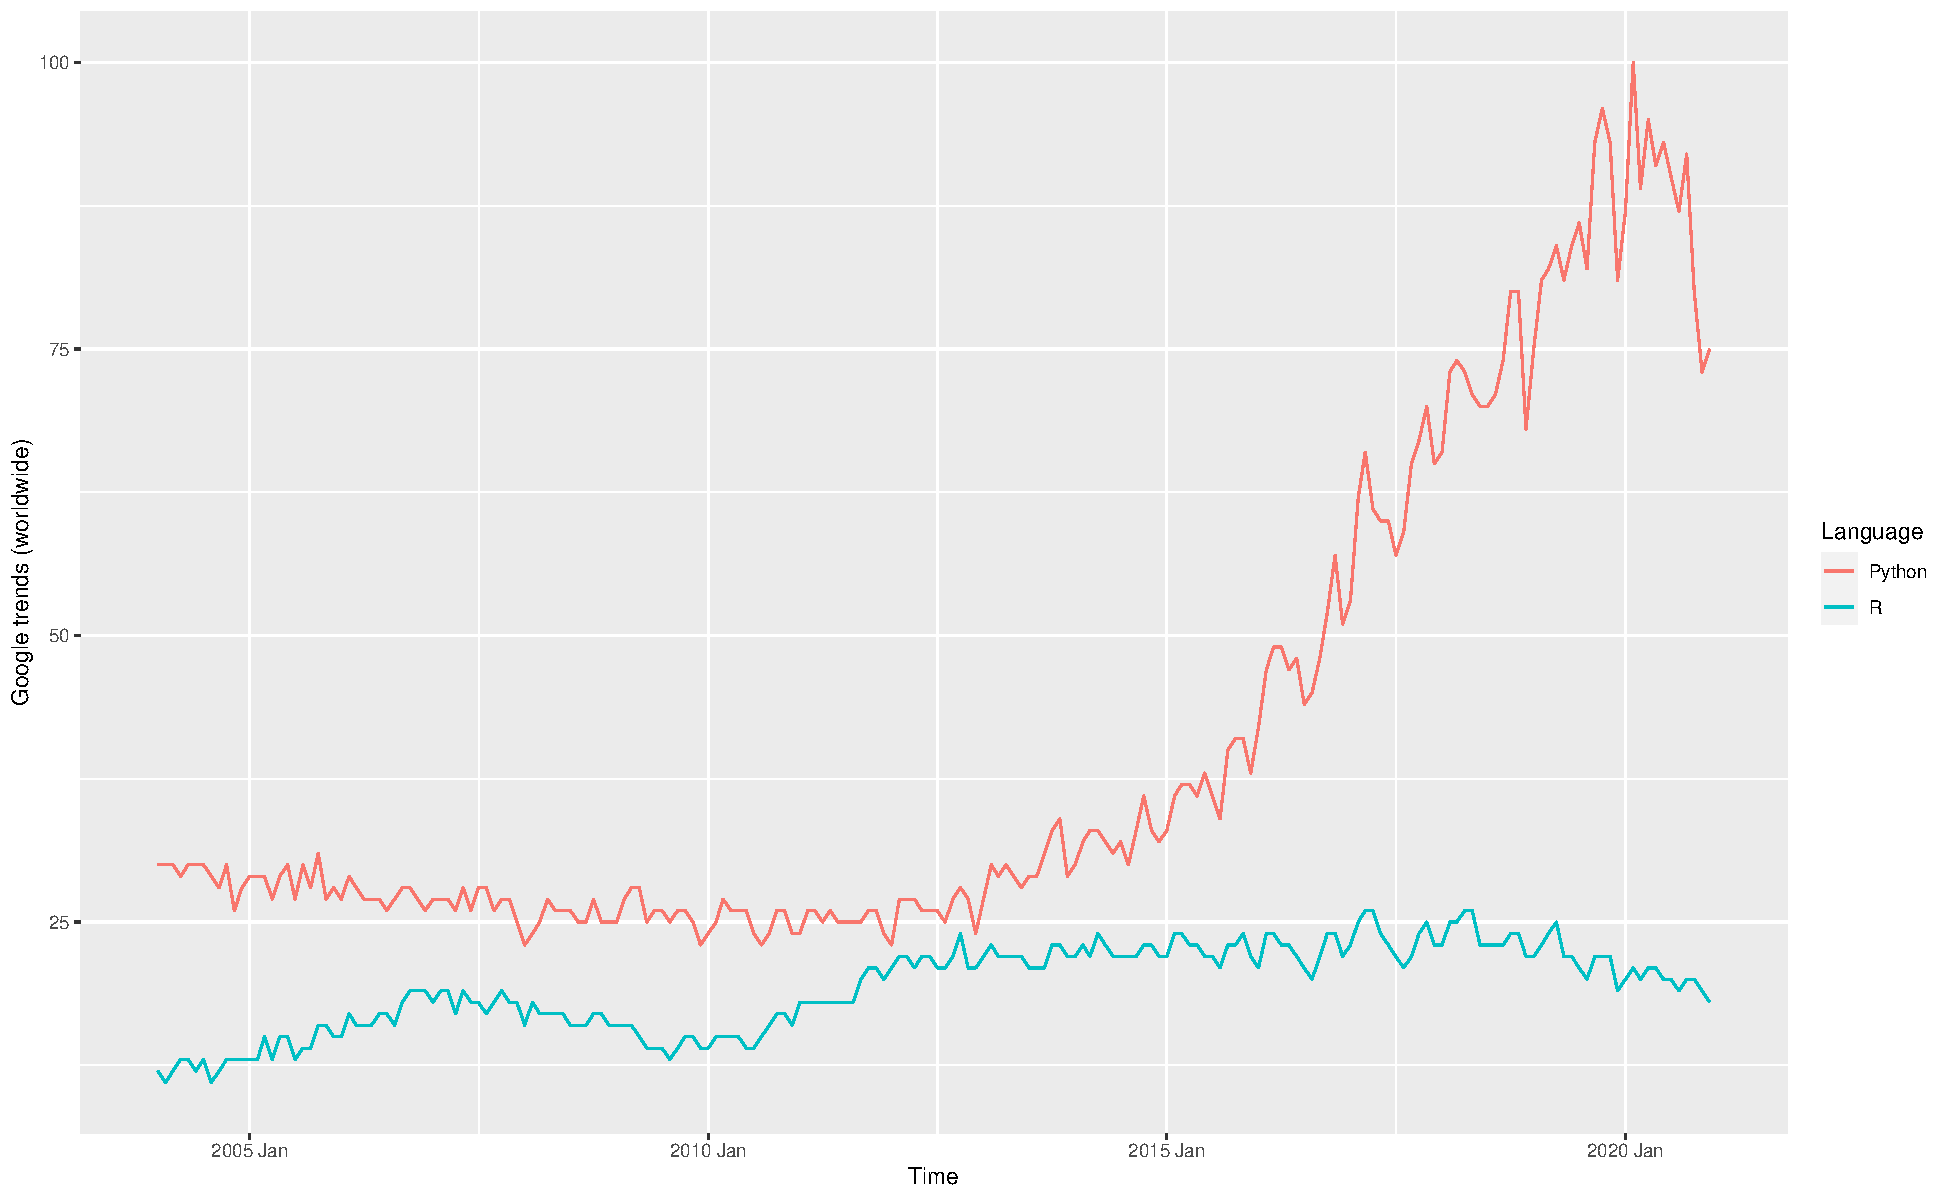
\includegraphics{bookdown-demo_files/figure-latex/googletrends-1.pdf}

\hypertarget{variables-expressions-and-statements}{%
\chapter{Variables, expressions, and statements}\label{variables-expressions-and-statements}}

WIP

\hypertarget{conditional-execution}{%
\chapter{Conditional execution}\label{conditional-execution}}

WIP

\hypertarget{functions}{%
\chapter{Functions}\label{functions}}

WIP

\hypertarget{iteration}{%
\chapter{Iteration}\label{iteration}}

\hypertarget{import}{%
\chapter{Import}\label{import}}

\hypertarget{tidy-clean-and-transform}{%
\chapter{Tidy: Clean and Transform}\label{tidy-clean-and-transform}}

\hypertarget{manipulate-transform-and-tidy}{%
\chapter{Manipulate, Transform and Tidy}\label{manipulate-transform-and-tidy}}

\hypertarget{visualize}{%
\chapter{Visualize}\label{visualize}}

\hypertarget{visualize-1}{%
\chapter{Visualize}\label{visualize-1}}

\hypertarget{communicate}{%
\chapter{Communicate}\label{communicate}}

\bibliography{book.bib}

\end{document}
